\documentclass{article}
\usepackage[utf8]{inputenc}
\usepackage[spanish]{babel}
\usepackage{amsmath}
\usepackage{amsfonts}
\usepackage{amssymb}
\usepackage{graphicx}
\usepackage[left=2cm,right=2cm,top=2cm,bottom=2cm]{geometry}
\usepackage{listings}
\usepackage[hidelinks]{hyperref}

\lstset {
    frame = single,
    breaklines = true
}



\begin{document}

\begin{titlepage}
\title{\textbf{
    {\Huge Ataque Mitnick}\\
    {\Large Seguridad Informática}
}}
\author{
    Pedro Allué Tamargo (758267)
    \and
    Juan José Tambo Tambo (755742)
}
\date{\today}
\clearpage\maketitle
\thispagestyle{empty}
\tableofcontents
\end{titlepage}

% Documento
\section{El Ataque \textit{Mitnick}}

El ataque \textit{Mitnick} es un tipo de Ataque \textit{TCP} que se aprovecha de las vulnerabilidades del protocolo. En este ataque \textit{Mitnick} explotó las vulnerabilidades del protocolo \textit{TCP} y la relación de confianza entre las dos máquinas de la víctima.\\
\textit{TCP} cuenta con un \textit{preprotocolo} llamado \textit{``saludo a tres bandas'' (three-way handshake)}. Este \textit{preprotocolo} verifica que la máquina con la que se está conectando es la que dice ser enviando una secuencia de números (\textit{sequence number}) con la que se debe realizar una operación matemática (suma) y enviarlo de vuelta al originario como \textit{ACK} (Figura \ref{fig:threewayhandshake}).\\
La red estaba compuesta por dos máquinas: un servidor verificado y la máquina \textit{``X-Terminal''} que era el objetivo. Para comunicarse con la máquina \textit{``X-Terminal''} se utilizaba el protocolo \textit{RSH\footnote{\url{https://es.wikipedia.org/wiki/Rsh}}}. Este protocolo utiliza dos conexiones \textit{TCP}, una para el envío de los comandos desde la máquina \textit{cliente} hacia la máquina \textit{servidor} y otra para el envío de mensajes de error desde la máquina \textit{servidor} al \textit{cliente}. Si la segunda conexión no está presente el servidor reiniciará la primera conexión (\textit{Flag RST} de \textit{TCP}). Este protocolo ya no se utiliza ya que ahora se utilizan opciones más seguras como \textit{SSH}.\\

Este ataque se divide en distintos pasos. El primero de ellos es la predicción de los números de secuencia iniciales de las conexiones \textit{TCP}. \textit{Mitnick} realizó envíos de paquetes \textit{SYN} y cuando la máquina \textit{``X-Terminal''} le contestaba con el número de secuencia este enviaba un mensaje con el \textit{flag RST} para reiniciar la conexión. Tras la repetición de este proceso 20 veces descubrió que existía un patrón entre 2 \textit{initial sequence numbers (ISN)} consecutivos.\\
Una vez averiguó el patrón de los números de secuencia, \textit{Mitnick} necesitaba silenciar al servidor verificado ya que si intentaba suplantar su identidad mientras este pudiera contestar enviaría un paquete \textit{TCP} con el \textit{flag RST} y reiniciaría la conexión. Para silenciarlo utilizó un ataque de denegación de servicio mediante una inundación de paquetes \textit{SYN}. Con este ataque el servidor verificado podría llegar a apagarse, de esta manera no enviaría el \textit{flag RST}.\\
El siguiente paso es suplantar la identidad del servidor verificado mediante una conexión \textit{TCP}. Para conseguir esto, \textit{Mitnick} envió un paquete \textit{TCP} con el \textit{flag SYN} a la máquina \textit{``X-Terminal''} pero poniendo como dirección de origen la del servidor verificado. Este servidor al estar apagado no podía resetear la conexión (\textit{flag RST}). La máquina \textit{``X-Terminal''} contestó a la petición con el mensaje \textit{SYN+ACK}. Este mensaje tenía un \textit{ISN} que \textit{Mitnick} no conocía pero que podía predecir utilizando la observación realizada anteriormente. \textit{Mitnick} contestó a este mensaje con un paquete con el \textit{flag ACK} y los números de secuencia y \textit{ACK} correspondientes. En el cuerpo del mensaje \textit{ACK} iba introducido el comando con el formato del protocolo \textit{RSH} para permitir el acceso sin contraseña a \textit{Mitnick} desde cualquier equipo.\\


\section{Configuración del entorno}

Se va a simular el entorno del ataque original. En este entorno existirán 3 máquinas: la máquina atacante, la máquina \textit{``X-Terminal''} (víctima) y el servidor verificado. Estas máquinas se encontrarán todas en la misma subred.\\
Se ha utilizado \textit{Docker} y \textit{Docker Compose} para simular el sistema. Las máquinas serán contenedores conectados bajo la red especificada en el orquestador \textit{Docker Compose}.\\
Cada una de las máquinas utiliza una imagen personalizada de \textit{Ubuntu} con \textit{RSH} instalado (Listing~\ref{listing:dockerfile}).\\
Para conectar las máquinas se ha utilizado la subred \textit{10.9.0.0/24} (Figura~\ref{fig:diagramaRed}). Para la orquestación del sistema se ha utilizado el fichero \textit{docker-compose.yml} del Listing~\ref{listing:docker-compose}. Se puede observar que el contenedor del atacante tiene un volumen en el que se monta el directorio \texttt{./volumes} en el directorio \texttt{/volumes} del contenedor. También se puede observar que el modo de red de este contenedor es \textit{host}, esto significa que el contenedor expondrá todos sus puertos como si estuviera siendo ejecutado en la máquina \textit{host}. Gracias a esto se podrá utilizar una herramienta de \textit{sniffing} de paquetes desde la máquina \textit{host} como si fuera la máquina atacante.\\

Para levantar el sistema se utilizará el comando \texttt{docker-compose up} y mediante los identificadores de los contenedores obtenidos con el comando \texttt{docker ps} se podrán ejecutar terminales para cada uno de los contenedores mediante el comando \texttt{docker exec -it \textit{id} /bin/bash}.\\

Para configurar el inicio de sesión vía \textit{RSH} sin contraseña desde el servidor verificado en la máquina \textit{``X-Terminal''} se van a ejecutar los siguientes comandos en la máquina \textit{víctima}:

\begin{lstlisting}
su seed
echo 10.9.0.6 >.rhosts
chmod 0644 .rhosts
\end{lstlisting}

Ahora el servidor seguro (con IP \textit{10.9.0.6}) podrá acceder vía \textit{RSH} sin la necesidad de introducir la contraseña desde el usuario \texttt{seed}.\\
Si se hubiera añadido la cadena \texttt{+ +} al fichero \texttt{.rhosts} podrían acceder todas las máquinas sin necesidad de contraseña.\\


\section{Realización del ataque} 

\subsection{Inundación de peticiones \textit{SYN} de \textit{Trusted Server}}

Para poder enviar una petición de conexión del servidor verificado al \textit{``X-Terminal''}, Mitnick debía enviar un paquete \textit{SYN} desde el servidor verificado al \textit{``X-Terminal''}, a lo que este respondería con un paquete de tipo \textit{SYN + ACK} hacia el servidor verificado. Como éste último no había comenzado la petición inicial, respondería con un paquete \textit{RESET} al \textit{``X-Terminal''}, indicando que finalizara el protocolo de sincronización (\textit{3-way handsake}, Figura \ref{fig:threewayhandshake}). De esta manera, era imposible poder realizar el ataque, por lo Mitnick necesitó ``silenciar'' al servidor verificado. Para ello, utilizó un ataque \textit{``Syn flooding''}\footnote{\url{https://en.wikipedia.org/wiki/SYN_flood}} (Figura \ref{fig:TCP-SYN-flood}) hacia el servidor verificado. Con ello consiguió apagar este servidor y, por tanto, silenciarlo completamente.\\

En la simulación, para simplificar el ataque \textit{SYN flooding}, se ha ``eliminado'' el servidor verificado parando el contenedor que simulaba este servidor mediante \texttt{sudo docker stop <ID\_CONTENEDOR>}.

Una vez silenciado el servidor verificado, si se realiza la petición \textit{SYN} a \textit{X-terminal}, este responderá con un paquete \textit{SYN + ACK}, para lo que necesita la dirección \textit{MAC} del servidor verificado. Primero se buscará en el caché \textit{ARP} y, en caso de que no haya ninguna entrada para el servidor verificado, se emitirá una petición \textit{ARP} para preguntar por esta \textit{MAC}. Como el servidor verificado está silenciado, no se emitirá una respuesta a esta petición, por lo que no se podrá establecer la conexión \textit{TCP}. En el ataque real, la máquina atacada si que tenía en caché la \textit{MAC} necesaria. Sin embargo, en la simulación se debe añadir la entrada de forma manual antes de silenciar el servidor verificado para que se almacene de forma permanente mediante el comando \texttt{arp -s [IP\_SERVER] [MAC\_SERVER]}.

\subsection{Primera conexión}
Una vez silenciado el servidor verificado, se procede a hacerse pasar este e intentar establecer una sesión \textit{rsh} con el \textit{``X-Terminal''}. Como \textit{rsh} funciona sobre el protocolo \textit{TCP}, en primer lugar se debe establecer una conexión \textit{TCP} entre el ``servidor verificado'' suplantado y el \textit{``X-Terminal''}. El problema principal de este paso era que tenían que predecir los números de secuencia de \textit{TCP}. Mitnick se aprovechó de que entonces no eran aleatorios (en la actualidad sí lo son) para poder predecir estos números. \\

En la simulación del ataque, se utiliza la herramienta \textit{WireShark} para observar la red y obtener estos números de secuencia. Los campos que se observarán serán: ``\textbf{Número secuencia \textit{TCP}}'' y `` \textbf{Tipo de paquete \textit{TCP}}''.\\

Una sesión \textit{rsh} consiste en dos conexiones de tipo \textit{TCP}. La primera se utiliza para el protocolo \textit{3-way handshake}. Una vez establecida la conexión, el cliente envía datos de \textit{rsh} al servidor destino. El proceso \textit{rshd} autentificará al cliente y, si se ha autenticado, se inicia una segunda conexión \textit{TCP}.
Esta segunda conexión se utiliza para enviar mensajes de error, la cual no interesa en el ataque, aunque se debe realizar ya que sino \textit{rshd} no continuará. Una vez se ha establecido la segunda conexión, el servidor destino enviará un byte \textit{``zero''} al cliente. Seguidamente, \textit{rshd} ejecutará el comando indicado por el cliente y la salida del mismo se enviará de vuelta al cliente (todo ello utilizando la primera conexión).\\

Para poder realizar el ataque, se deben establecer estas dos conexiones \textit{TCP}. Los pasos para establecer la primera (Figura \ref{fig:first-tcp-connection}) se explican a continuación.

\subsubsection{Mensaje \textit{SYN} a \textit{X-Terminal}}
En primer lugar, se debe enviar un falso paquete \textit{SYN} al \textit{X-Terminal}, haciéndose pasar por el servidor verificado. Para ello, se ha escrito un \textit{script} (ver código en \textit{listing }\ref{listing:script-syn}) en \textit{Python} utilizando la herramienta \textit{scapy}\footnote{\url{https://scapy.net/}} mediante la que se pueden mandar paquetes \textit{TCP}.\\

En el código se indica la \textit{IP} origen y destino de la comunicación (atacante a \textit{X-terminal}). Se puede observar que se utiliza como origen la IP que tenía el servidor verificado, ya que nos hacemos pasar por él. Además, se indica que el puerto origen es el 1023, ya que sino \textit{rsh} reiniciará la conexión una vez establecida\\
Antes de ejecutar el \textit{script}, se debe configurar \textit{Wireshark} para que observe los paquetes que recibe la máquina atacante. Para ello, ejecutamos \texttt{ip a} en esta máquina y observamos sus interfaces de red, concretamente en la que empieza por ``br-''. Desde \textit{Wireshark} se selecciona esta interfaz en el apartado \textit{Capture interfaces}. Además, se debe modificar la configuración de la herramienta para que no modifique los números de secuencia de la comunicación. Para ello, se accede a \texttt{Edit$\rightarrow$Preferences$\rightarrow$Protocols$\rightarrow$TCP} y se quita la casilla de \textit{``Relative secuence numbers''} \\

Si se ejecuta \textit{script} desde la máquina atacante, se puede observar en \textit{Wireshark} que se recibe un paquete de tipo \textit{SYN + ACK} desde la máquina víctima, respondiendo al servidor verificado (Figura \ref{fig:syn-wireshark}). De ese paquete interesa el campo \textit{Sequence number} par el siguiente paso. 

\subsubsection{Mensaje \textit{ACK} a \textit{X-Terminal}}
\label{section-ack}
Una vez recibido el mensaje \textit{SYN + ACK} por parte de \textit{X-Terminal}, el atacante debe contestar con un mensaje de tipo \textit{ACK}. Para ello, se ha desarrollado otro \textit{script} con \textit{Python} parecido al anterior (ver \textit{listing} \ref{listing:script-ack}). En este caso, el campo \textit{flag} es ``A'' para indicar que el mensaje es de tipo \textit{ACK}. Siguiendo el estándar del protocolo \textit{3-way Handshake} (Figura \ref{3-way-hs}), el campo \textit{seq} corresponde con el campo \textit{seq} indicado en el \textit{script} de \textit{SYN} anterior (\textit{listing \ref{listing:script-syn}}) más una unidad. Sin embargo, el campo \textit{ack} es \texttt{S + 1}, siendo \texttt{S} el valor obtenido en el campo \textit{Sequence number} mediante la captura de paquetes indicada en el punto anterior.\\
Con todo ello, el saludo a tres vías estaría completo, por lo que el atacante necesita enviar los datos \textit{rsh} a la víctima. Se puede observar que la línea 9 del \textit{listing \ref{listing:script-ack}) } indica estos datos de \textit{rsh}, los cuales cuentan con 4 partes: número de puerto, el \textit{ID} de usuario del cliente, \textit{ID} de usuario del servidor y el comando. El puerto será el utilizado en la segunda conexión (sección \ref{section-second-connect}). Los \textit{IDs} en los contenedores utilizados son \textit{seed}. Por último, el comando es la parte más importante del mensaje, ya que con ello se modifica el archivo \texttt{.rhosts} permitiendo que cualquier usuario con cualquier \textit{IP} pueda acceder al equipo atacado sin necesidad de utilizar contraseña. \\
Se puede observar que cada uno de los campos se separan con el Byte 0, añadiendo otro al final del mensaje.\\
Tras ejecutar este \textit{script}, si se analizan los paquetes capturados por \textit{Wireshark} (Figura \ref{fig:ack-wireshark}) se observa que se envían los datos \textit{RSH} desde la máquina atacante y la máquina atacada responde con un ultimo \textit{ACK}, tal y cómo se puede observar en la Figura \ref{fig:first-tcp-connection}. Además, se observa otro paquete que indica que la máquina atacada está intentando establecer comunicación con el puerto 9090 del ``servidor verificado'', tal y como se le ha indicado en los datos \textit{rsh}.

Seguidamente, si se analiza en la máquina atacada el archivo \texttt{.rhosts}, se observa que no ha sido modificado, es decir el comando indicado en los datos \textit{rsh} no se ha ejecutado. Esto se debe a que queda un último paso, establecer una segunda conexión \textit{TCP}.

\subsection{Segunda conexión}
\label{section-second-connect}

Una vez se ha establecido la primera conexión, se debe iniciar una segunda (Figura \ref{fig:second-tcp-connection}), que será utilizada por \textit{rshd} para mostrar los mensajes de error. Si no se realiza, el ataque no tendrá efecto ya que se cerrará la comunicación sin ejecutar el comando. \\

\subsubsection{Mensaje \textit{SYN+ACK} a \textit{X-Terminal}}

Como se ha indicado en la sección \ref{section-ack}, la máquina atacada intenta establecer una nueva conexión con el ``servidor verificado'' en el puerto 9090 al recibir un \textit{ACK}. A continuación, lo que se debe hacer es obtener el campo \textit{seq} del mensaje de \textit{SYN} de la máquina atacada para poder enviar un último paquete de tipo \textit{SYN + ACK} suplantando al servidor verificado y finalizar así el ataque.\\
Para ello, se ha desarrollado un tercer \textit{script} (\textit{listing} \ref{listing:script-syn-ack}) con el que se envía este paquete \textit{SYN + ACK} a la víctima, indicando que el puerto origen es 9090 (el mismo que en el mensaje \textit{ACK} anterior). El campo \textit{seq} no es importante, mientras que el de \textit{ack} debe ser el \textit{sequence number} obtenido del mensaje \textit{SYN} de la víctima más una unidad.\\

De esta manera, si se ejecuta el \textit{script} con los parámetros correctos y se analizan los paquetes capturados por \textit{Wireshark}, se observa el paquete \textit{SYN + ACK} enviado por el falso servidor verificado y el \textit{ACK} enviado de vuelta por parte de la víctima, además de dos mensajes de tipo \textit{FIN, ACK} que indican la finalización de la conexión. \\
Si se accede a la máquina atacada y se comprueba el archivo \texttt{.rhosts} (Figura \ref{fig:rhosts-after}), se ve que contiene ``+ +'', por lo que el comando indicado en el \textit{listing \ref{listing:script-ack}} se ha ejecutado correctamente. Por ello, ahora se podría acceder vía \textit{rsh} a la máquina víctima desde cualquier máquina sin necesidad de introducir contraseña, como se demuestra en la Figura \ref{fig:rsh-working}.

\section{Conclusiones}

Este ataque es muy interesante de cara a comprender como funciona el protocolo del \textit{three-way handshake} ya que en su tiempo se detectaron varias vulnerabilidades que se daban en el mismo. La primera vulnerabilidad es la capacidad de predecir los \textit{ISN (initial sequence numbers)} ya que dos peticiones consecutivas mostraban un patrón en estos números. Para solventar este problema, a día de hoy estos números son aleatorios, es decir, no siguen ningún patrón. Hoy en día para obtener este \textit{ISN} se utilizan herramientas como \textit{WireShark\footnote{\url{https://www.wireshark.org/}}} para observar la red y poder obtener estos números de secuencia.\\
La segunda vulnerabilidad se daba por la inundación de peticiones \textit{SYN} que se enviaban a la máquina segura. En esa época si una máquina recibía muchas peticiones de este tipo podía llegar a apagarse (ataque de denegación de servicio). \textit{Mitnick} se aprovechó de esta vulnerabilidad para llevar a cabo su ataque pero hoy en día esto no ocurre gracias a técnicas como el filtrado de los paquetes y otras contramedidas\footnote{\url{https://en.wikipedia.org/wiki/SYN_flood}}.\\
\textit{Mitnick} también se aprovechó del protocolo de comunicación \textit{RSH} que es capaz de lanzar una \textit{shell} en un equipo remoto. Este sistema transmitía los comandos en texto plano y eso presentaba un fallo de seguridad al permitir a todos los elementos de la red conocer la información que se transmitía. Esto permitió a \textit{Mitnick} enviar comandos vía \textit{TCP} siguiendo el protocolo de comunicación de \textit{RSH}. Hoy en día este sistema no se utiliza ya que existen alternativas seguras como \textit{SSH} que cifran la información que se transmite por la red.\\


\newpage
\addcontentsline{toc}{section}{Anexo 1: Figuras}
\section*{Anexo 1: Figuras}

\begin{figure}[htpb!]
    \centering
    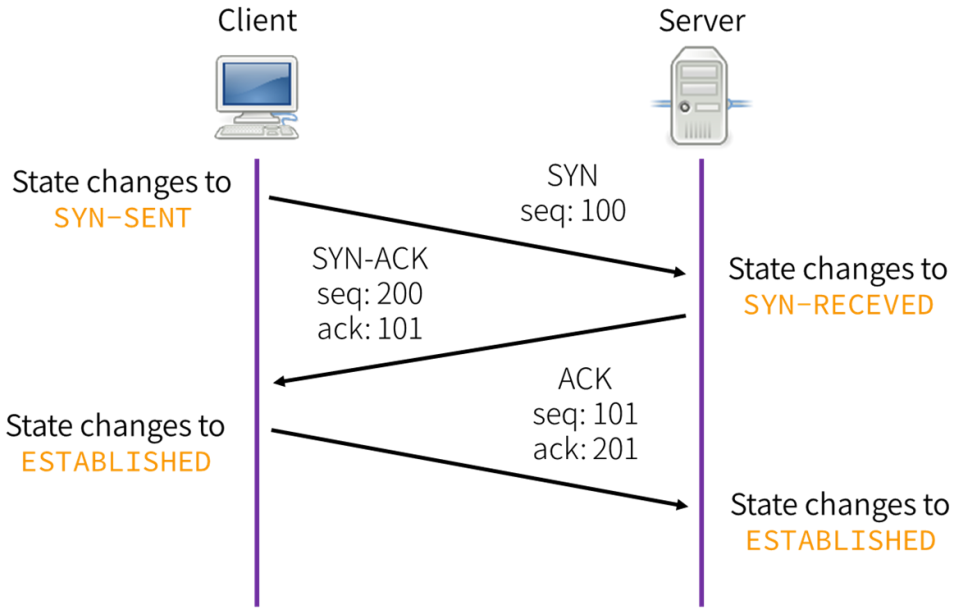
\includegraphics[scale=0.5]{images/threeway_handshake.png}
    \caption{Three-way Handshake protocol}
    \label{fig:threewayhandshake}
\end{figure}

\begin{figure}[htpb!]
    \centering
    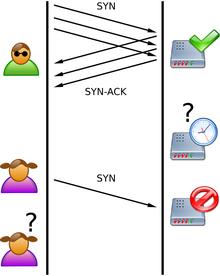
\includegraphics[scale=2]{images/Tcp_synflood.png}
    \caption{\textit{SYN flood} attack}
    \label{fig:TCP-SYN-flood}
\end{figure}

\begin{figure}[htpb!]
    \centering
    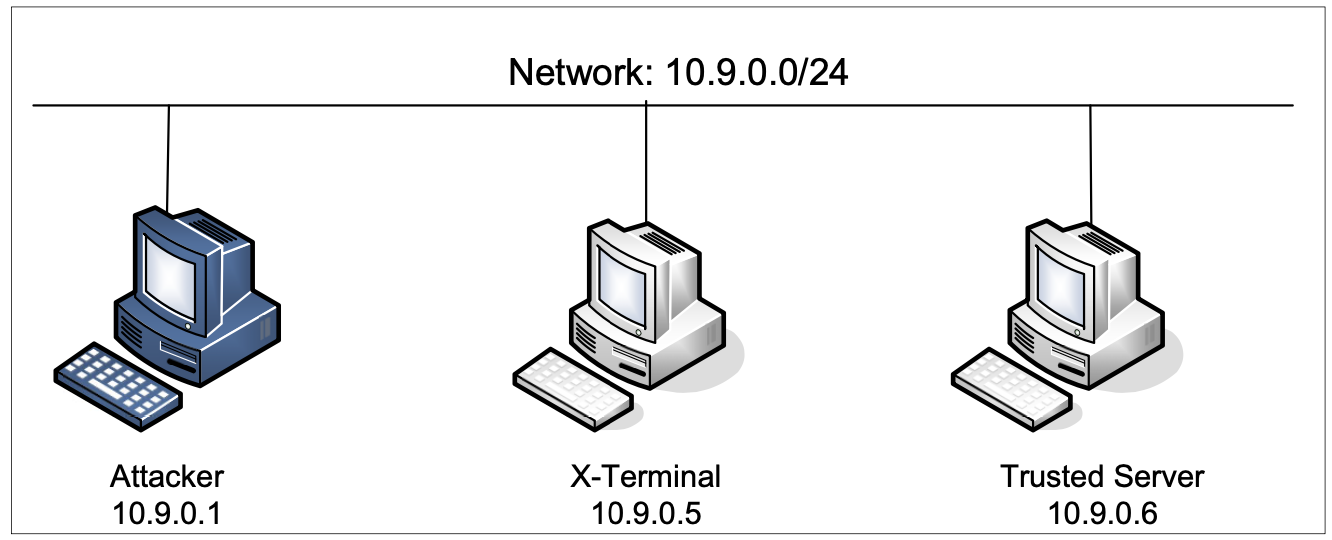
\includegraphics[scale=0.6]{images/diagramaRed.png}
    \caption{Diagrama de la red}
    \label{fig:diagramaRed}
\end{figure}

\begin{figure}[htpb!]
    \centering
    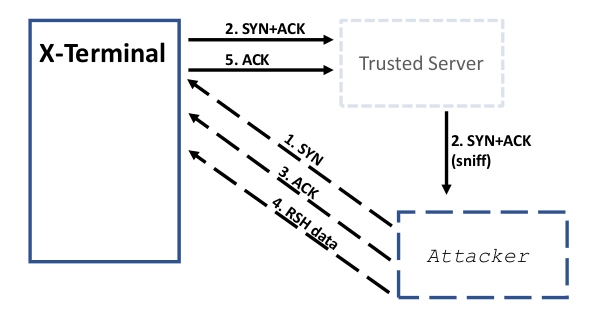
\includegraphics[scale=0.6]{images/first-tcp-connection.png}
    \caption{Primera conexión \textit{TCP}}
    \label{fig:first-tcp-connection}
\end{figure}

\begin{figure}[htpb!]
    \centering
    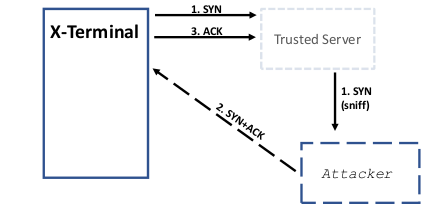
\includegraphics[scale=0.6]{images/second-tcp-connection.png}
    \caption{Segunda conexión \textit{TCP}}
    \label{fig:second-tcp-connection}
\end{figure}

\begin{figure}[htpb!]
    \centering
    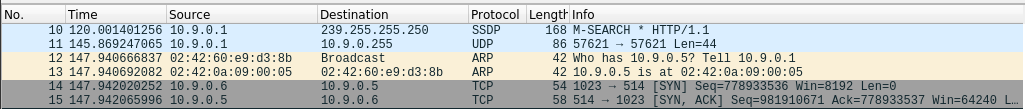
\includegraphics[scale=0.4]{images/syn-wireshark.png}
    \caption{Capturas de \textit{Wireshark} tras primer mensaje \textit{SYN}}
    \label{fig:syn-wireshark}
\end{figure}

\begin{figure}[htpb!]
    \centering
    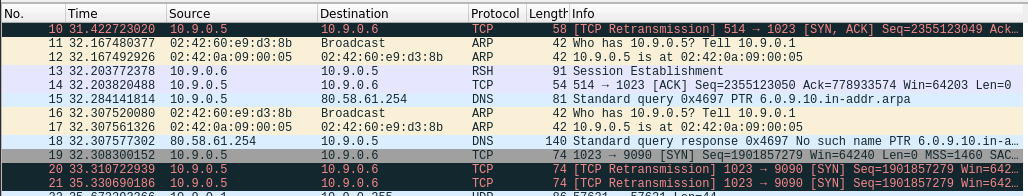
\includegraphics[scale=0.4]{images/ack-wireshark.png}
    \caption{Capturas de \textit{Wireshark} tras mensaje \textit{ACK}}
    \label{fig:ack-wireshark}
\end{figure}

\begin{figure}[htpb!]
    \centering
    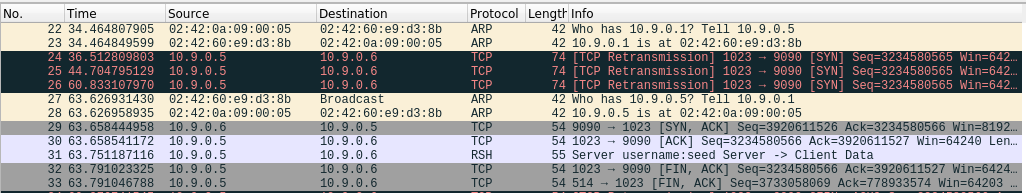
\includegraphics[scale=0.4]{images/syn-ack-wireshark.png}
    \caption{Capturas de \textit{Wireshark} tras mensaje \textit{SYN + ACK}}
    \label{fig:syn-ack-wireshark}
\end{figure}

\begin{figure}[htpb!]
    \centering
    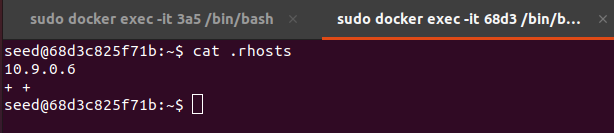
\includegraphics[scale=0.6]{images/rhosts-modified.png}
    \caption{Contenido de \textit{.rhosts} tras ataque \textit{Mitnick}}
    \label{fig:rhosts-after}
\end{figure}

\begin{figure}[htpb!]
    \centering
    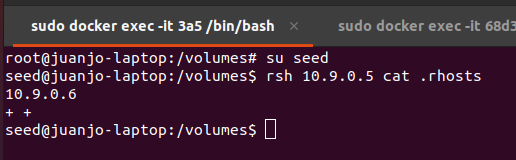
\includegraphics[scale=0.6]{images/rsh-work.png}
    \caption{Ejecución de \textit{rsh} desde máquina atacante sin autenticación}
    \label{fig:rsh-working}
\end{figure}


\newpage
\addcontentsline{toc}{section}{Anexo 2: Códigos}
\section*{Anexo 2: Códigos}

\subsection*{Fichero de creación de la imagen utilizada}

\lstinputlisting[label={listing:dockerfile}, caption={Fichero de creación de la imagen utilizada (\textit{Dockerfile})}]{listings/Dockerfile}

\subsection*{Fichero de configuración de \textit{Docker Compose}}

\lstinputlisting[label={listing:docker-compose}, caption={Fichero de configuración de \textit{Docker Compose}}]{listings/docker-compose.yml}

\subsection*{\textit{Script} para enviar paquete \textit{SYN}}

\lstinputlisting[label={listing:script-syn}, caption={\textit{Script} para comenzar la conexión \textit{TCP} enviando paquete \textit{SYN}}]{listings/script_syn.py}

\subsection*{\textit{Script} para enviar paquete \textit{ACK}}

\lstinputlisting[label={listing:script-ack}, caption={\textit{Script} para enviar paquete \textit{ACK} a \textit{X-Terminal}}]{listings/script_ack.py}

\newpage
\subsection*{\textit{Script} para enviar paquete \textit{SYN + ACK}}

\lstinputlisting[label={listing:script-syn-ack}, caption={\textit{Script} enviar mensaje \textit{SYN + ACK} para finalizar conexión}]{listings/script_syn_ack.py}
\end{document}
